\documentclass[10pt]{article}\usepackage[margin=.65in]{geometry}\usepackage[T1]{fontenc}\usepackage{graphicx}\setlength{\parindent}{0pt}\setlength{\parskip}{7pt}\sloppy\begin{document}{\large Next genus-2 interfaces: source derivations and fixed controls}\par Four parallel lanes produced source-bound constructions. These are written derivations, plus fixed native controls where stated, awaiting independent cross-review. No new scientific execution, cohort timing or cost ratio. The frozen1260-target scope remains unchanged.\par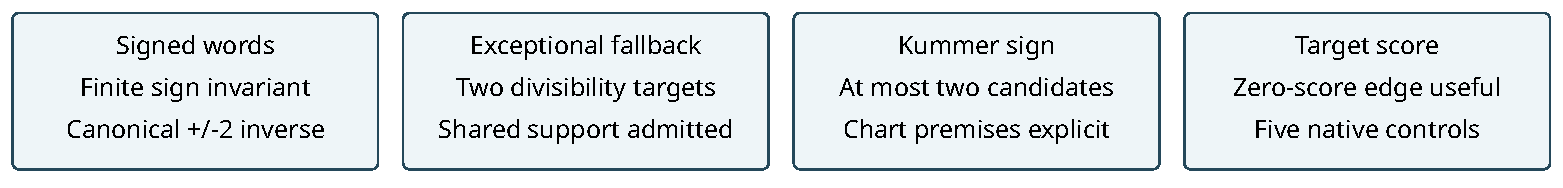
\includegraphics[width=\linewidth]{diagram.pdf}\par Signed words. Signs remain in plus/minus1 through find and union, with all intermediate i8 expressions representable. For odd scalar modulus r, inverse(+2)=r/2+1 and inverse(-2)=r/2. Canonical scalar addition needs r at most2\textasciicircum{}63. An invalid-sign source example shows why the caller sign premise cannot be removed. These algebraic reductions identify the remaining mutable-state refinement theorem.

Exceptional fallback. The extended-GCD construction tracks six registers, two Bezout equations and common divisors. At the actual two fallback call sites it derives that D squared divides UaUb and D divides the numerator N, including shared support and inverse pairs. Stored exact-division success still needs the new composed word theorem. The packet specifies malformed-input behavior and proposed controls, which were not executed.

Kummer sign. Given ordinary-chart correspondence S=b1 squared, the Mumford equations leave at most two opposite candidate divisors, including S=0. The adjacent projection relative to a non-two-torsion anchor determines orientation under the fiber premises. Opposite candidates give dependent rows. Eleven fixed native algebra assertions passed; neither a universal Lean chart theorem nor geometric enumeration is claimed.

Target score. Five fixed controls compiled the unchanged SignedGraph source over F7. A score-zero edge fixes u=0; the subsequent equation u=1+k then returns6 with score3. Without that edge the same equation scores2 and does not return. Current policy inserts all edges, so this is a distinction between immediate score and future usefulness. The first score call alone increments six scalar-add counts and two find visits. No insertion, constructor or timing cost is inferred from that diagnostic.

Evidence and review. Separate packets retain source hashes, assumptions, commands, outputs and structured obligations. Compiled binaries and preview/build intermediates are omitted from publication; original native receipts retain their hashes. Cross-review is assigned in PLAN.md after producer publication. The next implementation targets are mutable signed-word composition, extended-GCD fallback admission, coordinate-specific fiber correspondence and per-edge information accounting with score costs included.
\end{document}